
\documentclass[a4paper,11pt]{article}
\usepackage{amsmath,amsthm,amsfonts,amssymb,amscd,amstext,vmargin,graphics,graphicx,tabularx,multicol} \usepackage[french]{babel}
\usepackage[utf8]{inputenc}  
\usepackage[T1]{fontenc} 
\usepackage[T1]{fontenc}
\usepackage{amsmath,amssymb}
\usepackage{pstricks-add,tikz,tkz-tab,variations}
\usepackage[autolanguage,np]{numprint} 
\usepackage{color}
\usepackage{ulem}

\setmarginsrb{1.5cm}{0.5cm}{1cm}{0.5cm}{0cm}{0cm}{0cm}{0cm} %Gauche, haut, droite, haut
\newcounter{numexo}
\newcommand{\exo}[1]{\stepcounter{numexo}\noindent{\bf Exercice~\thenumexo} : \marginpar{\hfill /#1}}
\reversemarginpar


\newcounter{enumtabi}
\newcounter{enumtaba}
\newcommand{\q}{\stepcounter{enumtabi} \theenumtabi.  }
\newcommand{\qa}{\stepcounter{enumtaba} (\alph{enumtaba}) }
\newcommand{\initq}{\setcounter{enumtabi}{0}}
\newcommand{\initqa}{\setcounter{enumtaba}{0}}

\newcommand{\be}{\begin{enumerate}}
\newcommand{\ee}{\end{enumerate}}
\newcommand{\bi}{\begin{itemize}}
\newcommand{\ei}{\end{itemize}}
\newcommand{\bp}{\begin{pspicture*}}
\newcommand{\ep}{\end{pspicture*}}
\newcommand{\bt}{\begin{tabular}}
\newcommand{\et}{\end{tabular}}
\renewcommand{\tabularxcolumn}[1]{>{\centering}m{#1}} %(colonne m{} centrée, au lieu de p par défault) 
\newcommand{\tnl}{\tabularnewline}

\newcommand{\trait}{\noindent \rule{\linewidth}{0.2mm}}
\newcommand{\hs}[1]{\hspace{#1}}
\newcommand{\vs}[1]{\vspace{#1}}

\newcommand{\N}{\mathbb{N}}
\newcommand{\Z}{\mathbb{Z}}
\newcommand{\R}{\mathbb{R}}
\newcommand{\C}{\mathbb{C}}
\newcommand{\Dcal}{\mathcal{D}}
\newcommand{\Ccal}{\mathcal{C}}
\newcommand{\mc}{\mathcal}

\newcommand{\vect}[1]{\overrightarrow{#1}}
\newcommand{\ds}{\displaystyle}
\newcommand{\eq}{\quad \Leftrightarrow \quad}
\newcommand{\vecti}{\vec{\imath}}
\newcommand{\vectj}{\vec{\jmath}}
\newcommand{\Oij}{(O;\vec{\imath}, \vec{\jmath})}
\newcommand{\OIJ}{(O;I,J)}

\newcommand{\bmul}[1]{\begin{multicols}{#1}}
\newcommand{\emul}{\end{multicols}}


\newcommand{\reponse}[1][1]{%
\multido{}{#1}{\makebox[\linewidth]{\rule[0pt]{0pt}{20pt}\dotfill}
}}

\newcommand{\titre}[5] 
% #1: titre #2: haut gauche #3: bas gauche #4: haut droite #5: bas droite
{
\noindent #2 \hfill #4 \\
#3 \hfill #5

\vspace{-1.6cm}

\begin{center}\rule{6cm}{0.5mm}\end{center}
\vspace{0.2cm}
\begin{center}{\large{\textbf{#1}}}\end{center}
\begin{center}\rule{6cm}{0.5mm}\end{center}
}



\begin{document}
\pagestyle{empty}
\titre{Devoir maison}{Nom :}{Prénom :}{3 ème}{Date :}

\vspace*{1cm}

\exo

\textit{Toutes vos réponses devront être justifiées, soit par construction soit par démonstration. }\\


\vspace*{0.5cm}

Dans cette partie, on considère un triangle ABC de dimensions quelconques. \\ 

On appelle :\\

\hspace*{2.4cm}- B' le symétrique de B par rapport au milieu I de [AC].\\
\hspace*{3cm}- C' le symétrique de C par rapport au milieu J de [AB].\\
\hspace*{3cm}- A' l'intersection des droites (C'B) et (B'C).\\

A chaque question, on pourra utiliser le résultat d'une question précédente, même si celui-ci n'a pas été démontré.\\

\q \begin{center}
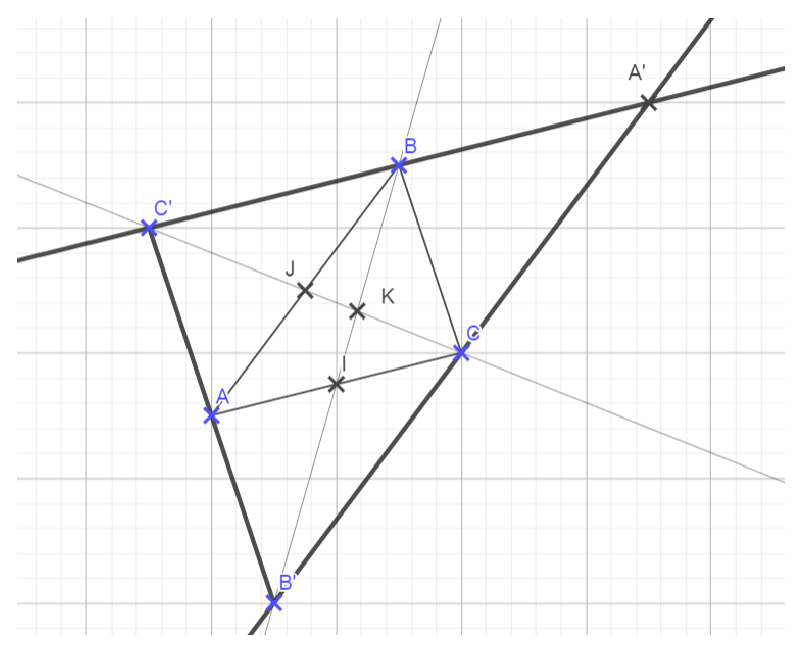
\includegraphics[scale=0.6]{imagedmparallelogramme.eps} 
\end{center}

\q 
Dans le quadrilatère ABCB'.\\
On sait que I est le milieu de [AC].\\
Par construction, B' est le symétrique de B par rapport à I. Autrement dit, I est le milieu aussi de [AC].\\

Or, un quadrilatère dont les diagonales se coupent en leur milieu est un parallélogramme.\\

Donc ABCB' est un parallélogramme et par définition, on peut affirmer que (AB) est parallèle à (B'C).\\


\q D'une part, puisque ABCB' est un parallélogramme, nous pouvons affirmer que (AB’) est parallèle à (BC).\\
D'autre part, le raisonnement de la question précédente s'applique au quadrilatère ACBC’ qui est donc un parallélogramme, d'où l'on déduit que (C'A) et (BC) sont parallèles entre elles.\\

Ainsi, les deux droites (C'A) et (AB') sont parallèles à (BC) et passent par un point commun, A.\\
D'après le principe d'Euclide, on ne peut mener par A qu'une seule parallèle à (BC). On en conclut donc que les droites (C'A) et (AB') sont confondues, autrement dit que les trois points C', A et B' sont alignés.\\

\q 
Puisque ABCB' est un parallélogramme, nous pouvons affirmer que BC = AB'.\\
De même ACBC' est un parallélogramme, donc BC = AC'.\\

Or, BC = AB' et BC = AC', on a donc AB' = AC'.\\
Les points A, B' et C' étant alignés ont peut affirmer que A est le milieu du segment [C'B']\\

\q Montrer que le point C est le milieu du segment [A'B'].\\

Il n'est pas nécessaire de refaire les démonstrations, le raisonnement s'applique de la même manière aux parallélogrammes ABA’C, ABCB’. \\

D'où, BA = B'C et BA = CA' donc B'C = CA' et les points B', C et A sont alignés donc le point C est bien le milieu du segment [A'B'].\\

\q D'après les questions précédentes, B et C sont les milieux de deux côtés du triangle A’B’C’.\\
Donc (CC’) et (BB’) sont deux médianes du triangle A’B’C’.\\

Or les 3 médianes d'un triangle sont concourantes en un point, ici K que l'on appelle le centre de gravité du triangle. \\

De fait, la droite (AA') est la 3ème médiane du triangle et elle passe par le point K. On peut en conclure que les points A, K et A' sont bien alignés.\\


\q Les 3 triangles sont A’B’C’, ABC et IJL, en appelant L le milieu de [BC].\\
En effet, ces trois triangles ont les mêmes droites médianes.\\

\vspace*{0.5cm}


\exo 

On donne l'expression suivante : $A=64 - (x-3)^2$\\

\initq
\noindent \q Calculer la valeur de $A$ lorsque $x=3$.\\

$A=64 - (3-3)^2$\\
$A=64 - (0)^2$\\
\fbox{$A=64$}\\

\noindent \q Développer et réduire l'expression $A$ à l'aide des identités remarquables.\\

$A=64 - (x-3)^2$\\
$A=64 - (x^{2} -6x + 9)$\\
$A=64 - x^{2} +6x - 9)$\\
\fbox{$A =-x^{2} + 6x + 55$}\\


 \q Utilise le résultat de la question précédente pour calculer la valeur de $A$ lorsque $x=3$. Que remarque-t-on? \\
 
$A =-3^{2} + 6 \times 3 + 55$\\
$A =-9 + 18 + 55$\\
\fbox{$A=64$}\\ 

 Les résultats sont identiques puisque $A=64 - (x-3)^2 $ et $A =-x^{2} + 6x + 55$\\


\end{document}
